\documentclass[a4paper,5pt]{amsbook}
%%%%%%%%%%%%%%%%%%%%%%%%%%%%%%%%%%%%%%%%%%%%%%%%%%%%%%%%%%%%%%%%%%%%%

%\usepackage{booktabs}
\usepackage{graphicx}
%\usepackage{multicol}
%\usepackage{textcomp}
%\usepackage{systeme}
%\usepackage{amssymb}
%\usepackage[]{amsmath}
%\usepackage{subcaption}
\usepackage[inline]{enumitem}
%\usepackage{gensymb}

%%%%%%%%%%%%%%%%%%%%%%%%%%%%%%%%%%%%%%%%%%%%%%%%%%%%%%%%%%%%%%

\newcommand{\sen}{\,\mbox{sen}\,}
\newcommand{\tg}{\,\mbox{tg}\,}
\newcommand{\cosec}{\,\mbox{cosec}\,}
\newcommand{\cotg}{\,\mbox{cotg}\,}
\newcommand{\tr}{\,\mbox{tr}\,}
\newcommand{\ds}{\displaystyle}
\newcommand{\ra}{\rightarrow}

%%%%%%%%%%%%%%%%%%%%%%%%%%%%%%%%%%%%%%%%%%%%%%%%%%%%%%%%%%%%%%%%%%%%%%%%

\setlength{\textwidth}{16cm} \setlength{\topmargin}{-1.7cm}
\setlength{\textheight}{25cm}
\setlength{\leftmargin}{1.2cm} \setlength{\rightmargin}{1.2cm}
\setlength{\oddsidemargin}{0cm}\setlength{\evensidemargin}{0cm}

%%%%%%%%%%%%%%%%%%%%%%%%%%%%%%%%%%%%%%%%%%%%%%%%%%%%%%%%%%%%%%%%%%%%%%%%

% \renewcommand{\baselinestretch}{1.6}
% \renewcommand{\thefootnote}{\fnsymbol{footnote}}
% \renewcommand{\theequation}{\thesection.\arabic{equation}}
% \setlength{\voffset}{-50pt}
% \numberwithin{equation}{chapter}

%%%%%%%%%%%%%%%%%%%%%%%%%%%%%%%%%%%%%%%%%%%%%%%%%%%%%%%%%%%%%%%%%%%%%%%

\begin{document}
\thispagestyle{empty}
\pagestyle{empty}
\begin{minipage}[h]{0.14\textwidth}
	
\includegraphics[scale=0.24]{../../ufgd.png}
\end{minipage}
\begin{minipage}[h]{\textwidth}
\begin{tabular}{c}
{{\bf UNIVERSIDADE FEDERAL DA GRANDE DOURADOS}}\\
{{\bf C\'alculo Diferencial e Integral --- Lista 9}}\\
{{\bf Prof.\ Adriano Barbosa}}\\
\end{tabular}
\vspace{-0.45cm}
%
\end{minipage}

%------------------------

\vspace{1cm}
%%%%%%%%%%%%%%%%%%%%%%%%%%%%%%%%   formulario  inicio  %%%%%%%%%%%%%%%%%%%%%%%%%%%%%%%%
\begin{enumerate}
    \vspace{0.5cm}
    \item Estime a \'area abaixo do gr\'afico de $f(x)=\cos{x}$ de $x=0$ at\'e
        $x=\ds\frac{\pi}{2}$ usando quatro ret\^angulos aproximantes usando os
        extremos direitos dos subintervalos. Repita o c\'alculo usando os
        extremos esquerdos dos subintervalos.

    \vspace{0.5cm}
    \item A velocidade de um corredor aumenta regularmente durante os tr\^es
        primeiros segundos de uma corrida. Sua velocidade em intervalos de
        meio segundo \'e dada pela tabela abaixo. Encontre as estimativas
        superior e inferior para a dist\^ancia que ele percorreu durante esses
        tr\^es segundos.

        \vspace{0.3cm}
        \begin{center}
        \begin{tabular}{|c|c|c|c|c|c|c|c|}
            \hline
            $t$ (s) & 0 & 0,5 & 1,0 & 1,5 & 2,0 & 2,5 & 3,0 \\
            \hline
            $v$ (m/s) & 0 & 1,9 & 3,3 & 4,5 & 5,5 & 5,9 & 6,2 \\
            \hline
        \end{tabular}
        \end{center}

    \vspace{0.5cm}
    \item O gr\'afico de $g$ consiste em duas retas e um semic\'{i}rculo. Use-o
        para calcular cada integral

    \begin{enumerate*}
    	\item $\displaystyle\int_0^2 g(x)\ dx$
        \hspace{0.3cm}
        \hspace{0.3cm}
    	\item $\displaystyle\int_2^6 g(x)\ dx$
        \hspace{0.3cm}
        \hspace{0.3cm}
    	\item $\displaystyle\int_0^6 g(x)\ dx$
    \end{enumerate*}
    
    \begin{figure}[h]
    	\centering
    	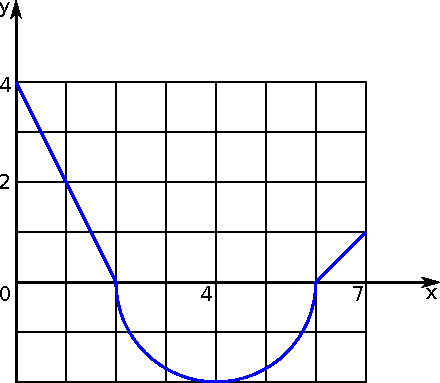
\includegraphics[scale=0.7]{lista-09-fig1.pdf}
    \end{figure}
    
    \vspace{0.5cm}
    \item Calcule as integrais interpretando-as em termos de \'areas.

    \begin{enumerate*}
    	\item $\displaystyle\int_{-1}^2 1 - x\ dx$
        \hspace{0.3cm}
        \hspace{0.3cm}
    	\item $\displaystyle\int_{-1}^2 |x|\ dx$
    \end{enumerate*}
    
    \vspace{0.5cm}
    \item Apenas analisando o gr\'afico das fun\c{c}\~oes, calcule as seguintes integrais

    \begin{enumerate*}
    	\item $\displaystyle\int_{-1}^1 x\ dx$
        \hspace{0.1cm}
        \hspace{0.1cm}
    	\item $\displaystyle\int_{-1}^1 |t|\ dt$
        \hspace{0.1cm}
        \hspace{0.1cm}
    	\item $\displaystyle\int_{-1}^1 y^2\ dy$
        \hspace{0.1cm}
        \hspace{0.1cm}
    	\item $\displaystyle\int_{-\pi}^{\pi} \sin\theta\ d\theta$
        \hspace{0.1cm}
        \hspace{0.1cm}
    	\item $\displaystyle\int_{-\pi}^{\pi} \cos\phi\ d\phi$
    \end{enumerate*}
\end{enumerate}

\end{document}
